\documentclass{article}
\usepackage[utf8]{inputenc}
\usepackage{amstext}
\usepackage{amsmath}
\usepackage{amsfonts}
\usepackage{graphicx}
\usepackage[margin=1in, paperwidth=8.5in, paperheight=11in]{geometry}
\usepackage{gensymb}
\usepackage{indentfirst}
\usepackage{textcomp}
\usepackage{upgreek }
\usepackage{siunitx}
\usepackage{enumitem}
\usepackage{epstopdf}
\epstopdfsetup{update} % only regenerate pdf files when eps file is newer

\usepackage[american]{circuitikz}

\title{Adaptive-Biasing Differential Amplifier}
\author{Byron Wasti}
\date{April 2017}

\begin{document}
\maketitle

\section{Introduction}

\section{Subtraction Sub-Circuit}

\begin{figure}[ht!]
    \centering
    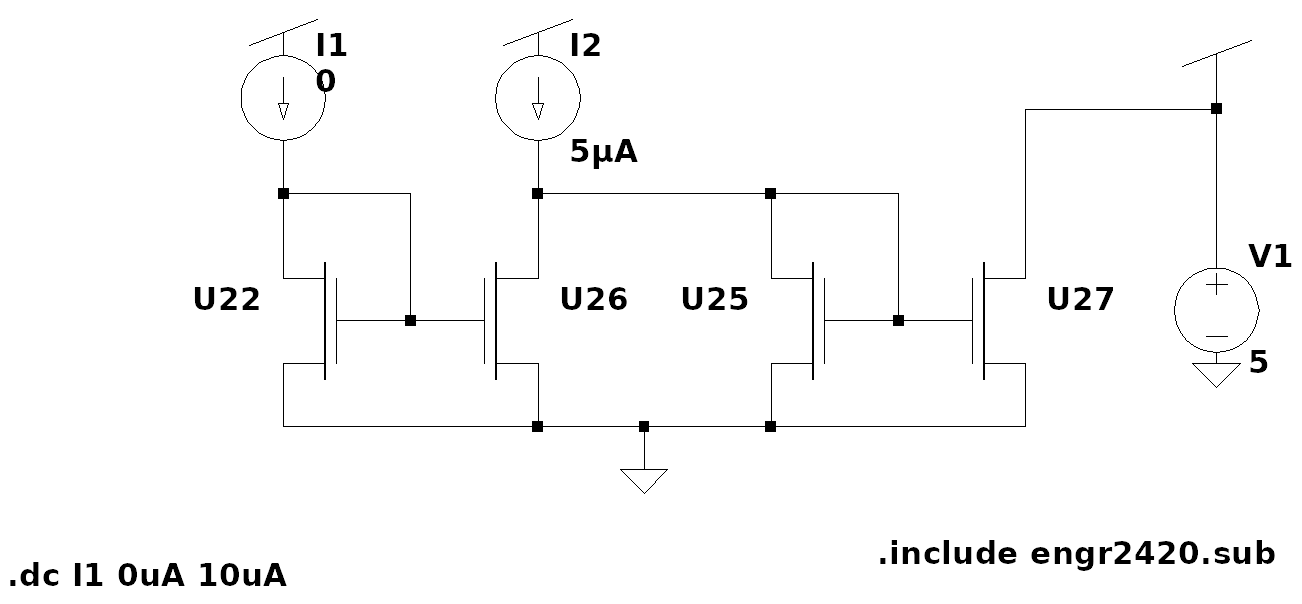
\includegraphics[width=\textwidth]{../Plots/subtractor_schem.png}
    \caption{Subtractor schematic.}
    \label{fig:postlab9}
\end{figure}

\begin{figure}[ht!]
    \centering
    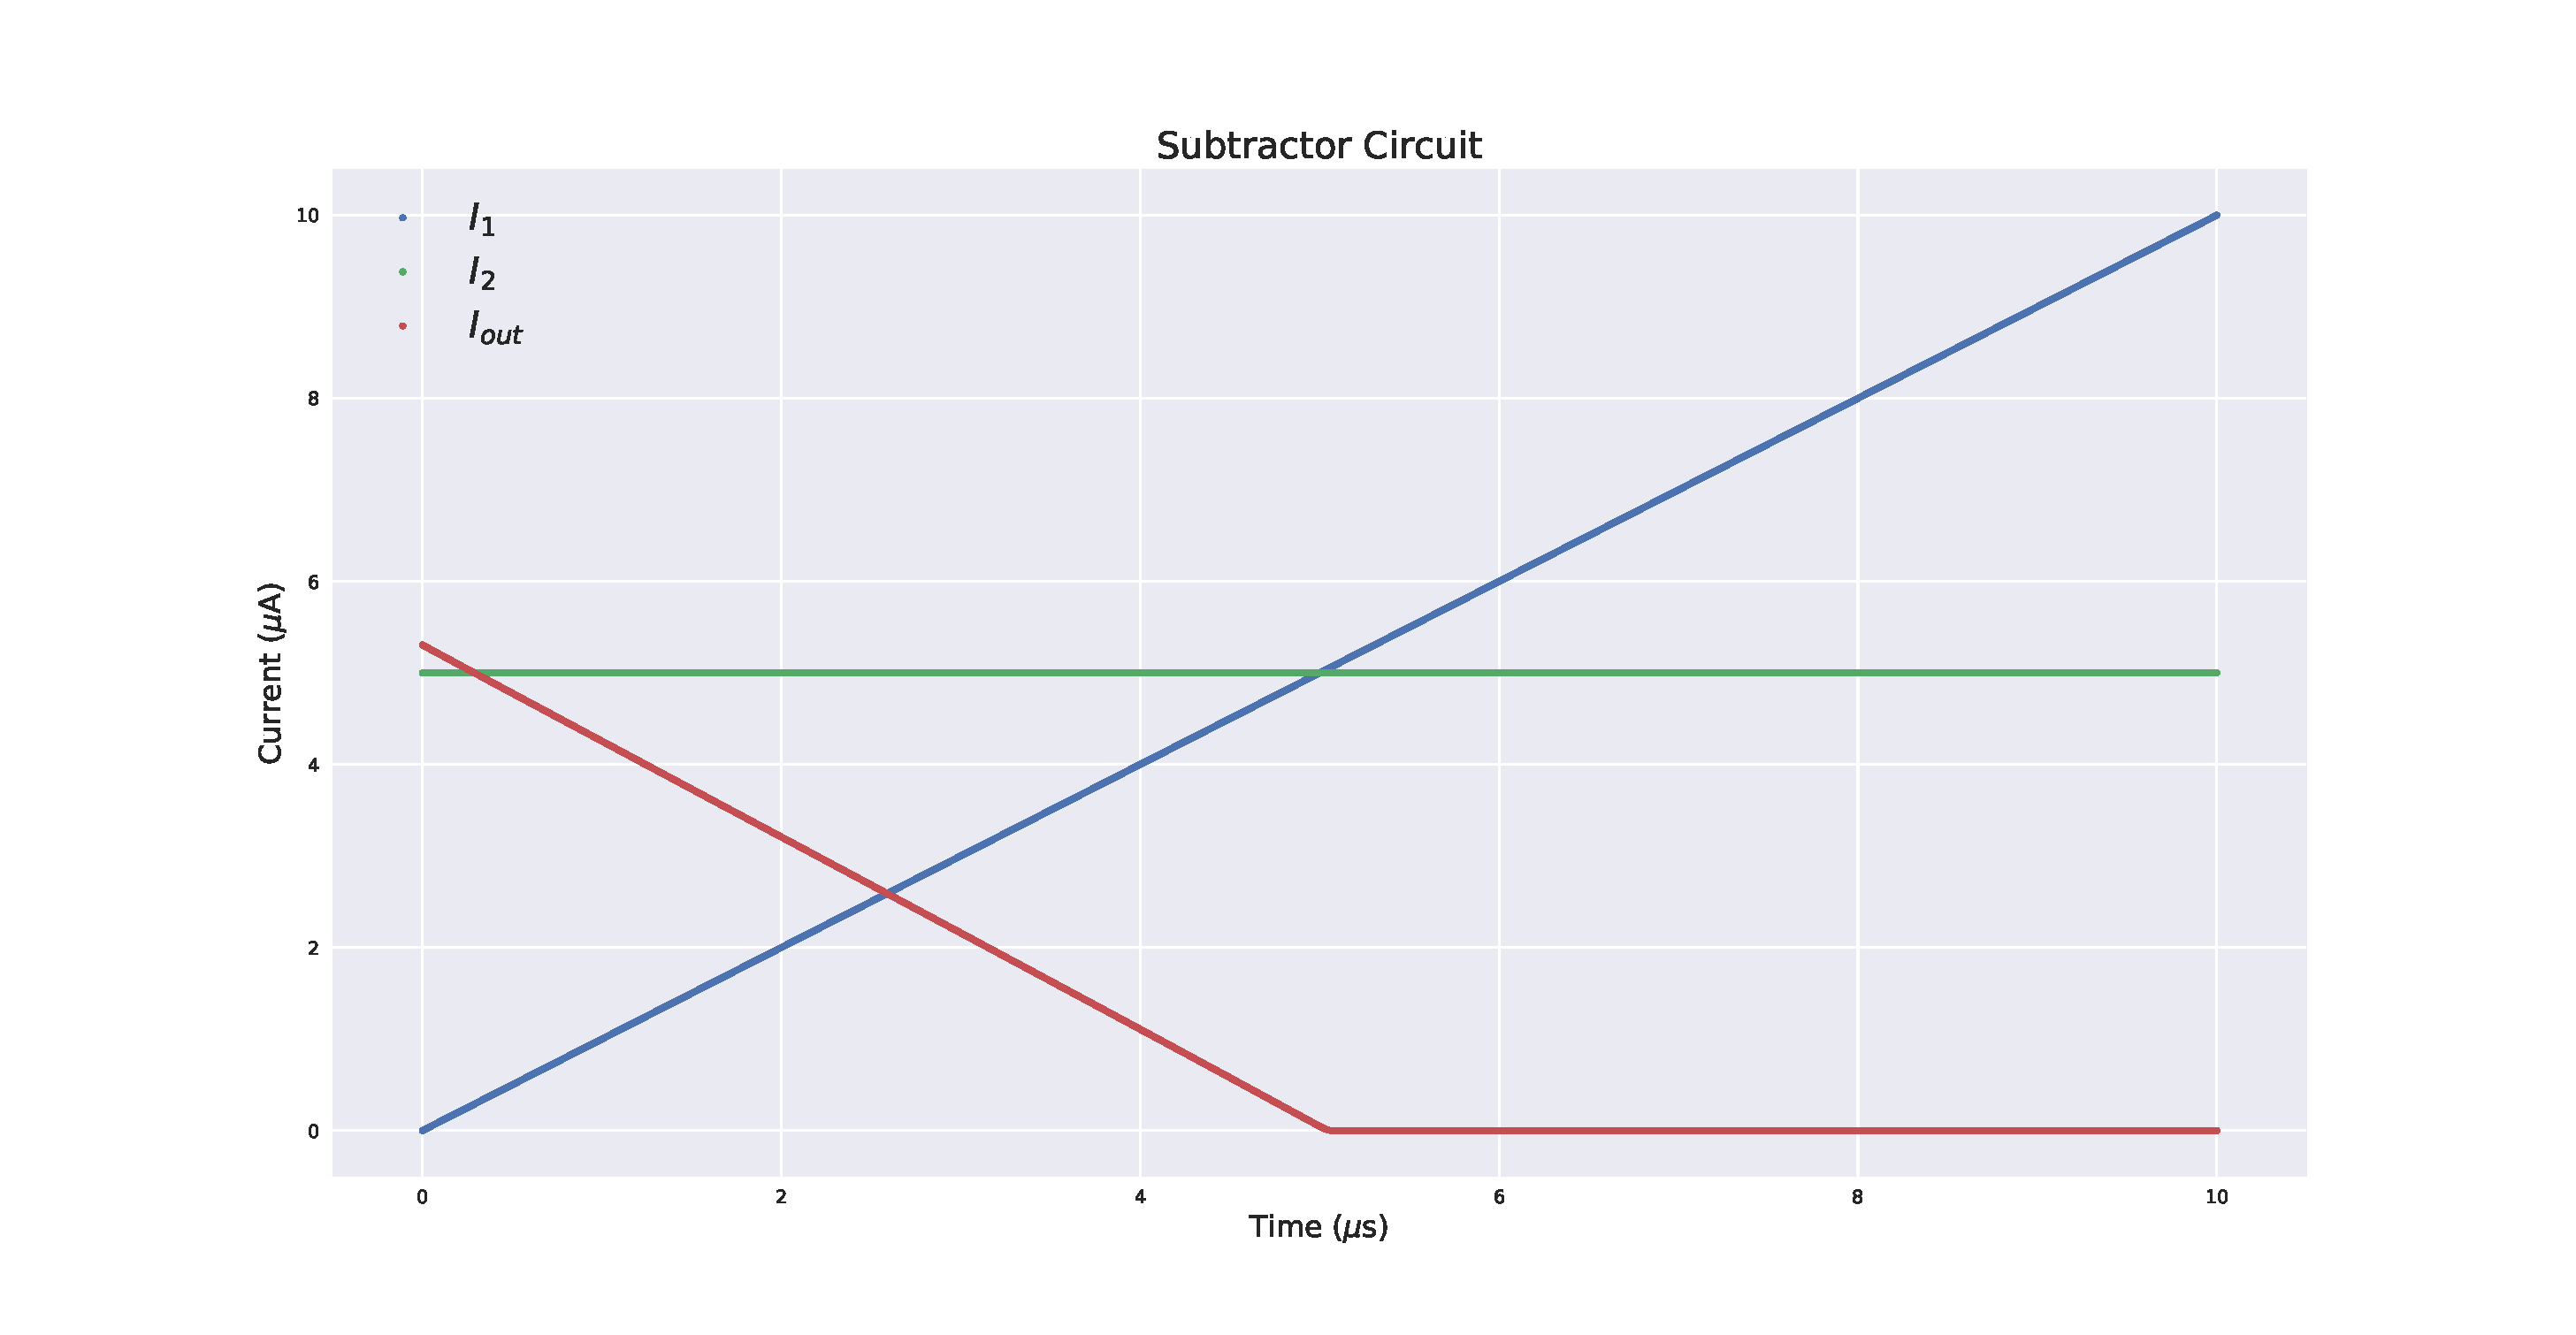
\includegraphics[width=\textwidth]{subtractor}
    \caption{Subtractor circuit input response.}
    \label{fig:postlab9}
\end{figure}


\section{Slew Rate Comparison}


\begin{figure}[ht!]
    \centering
    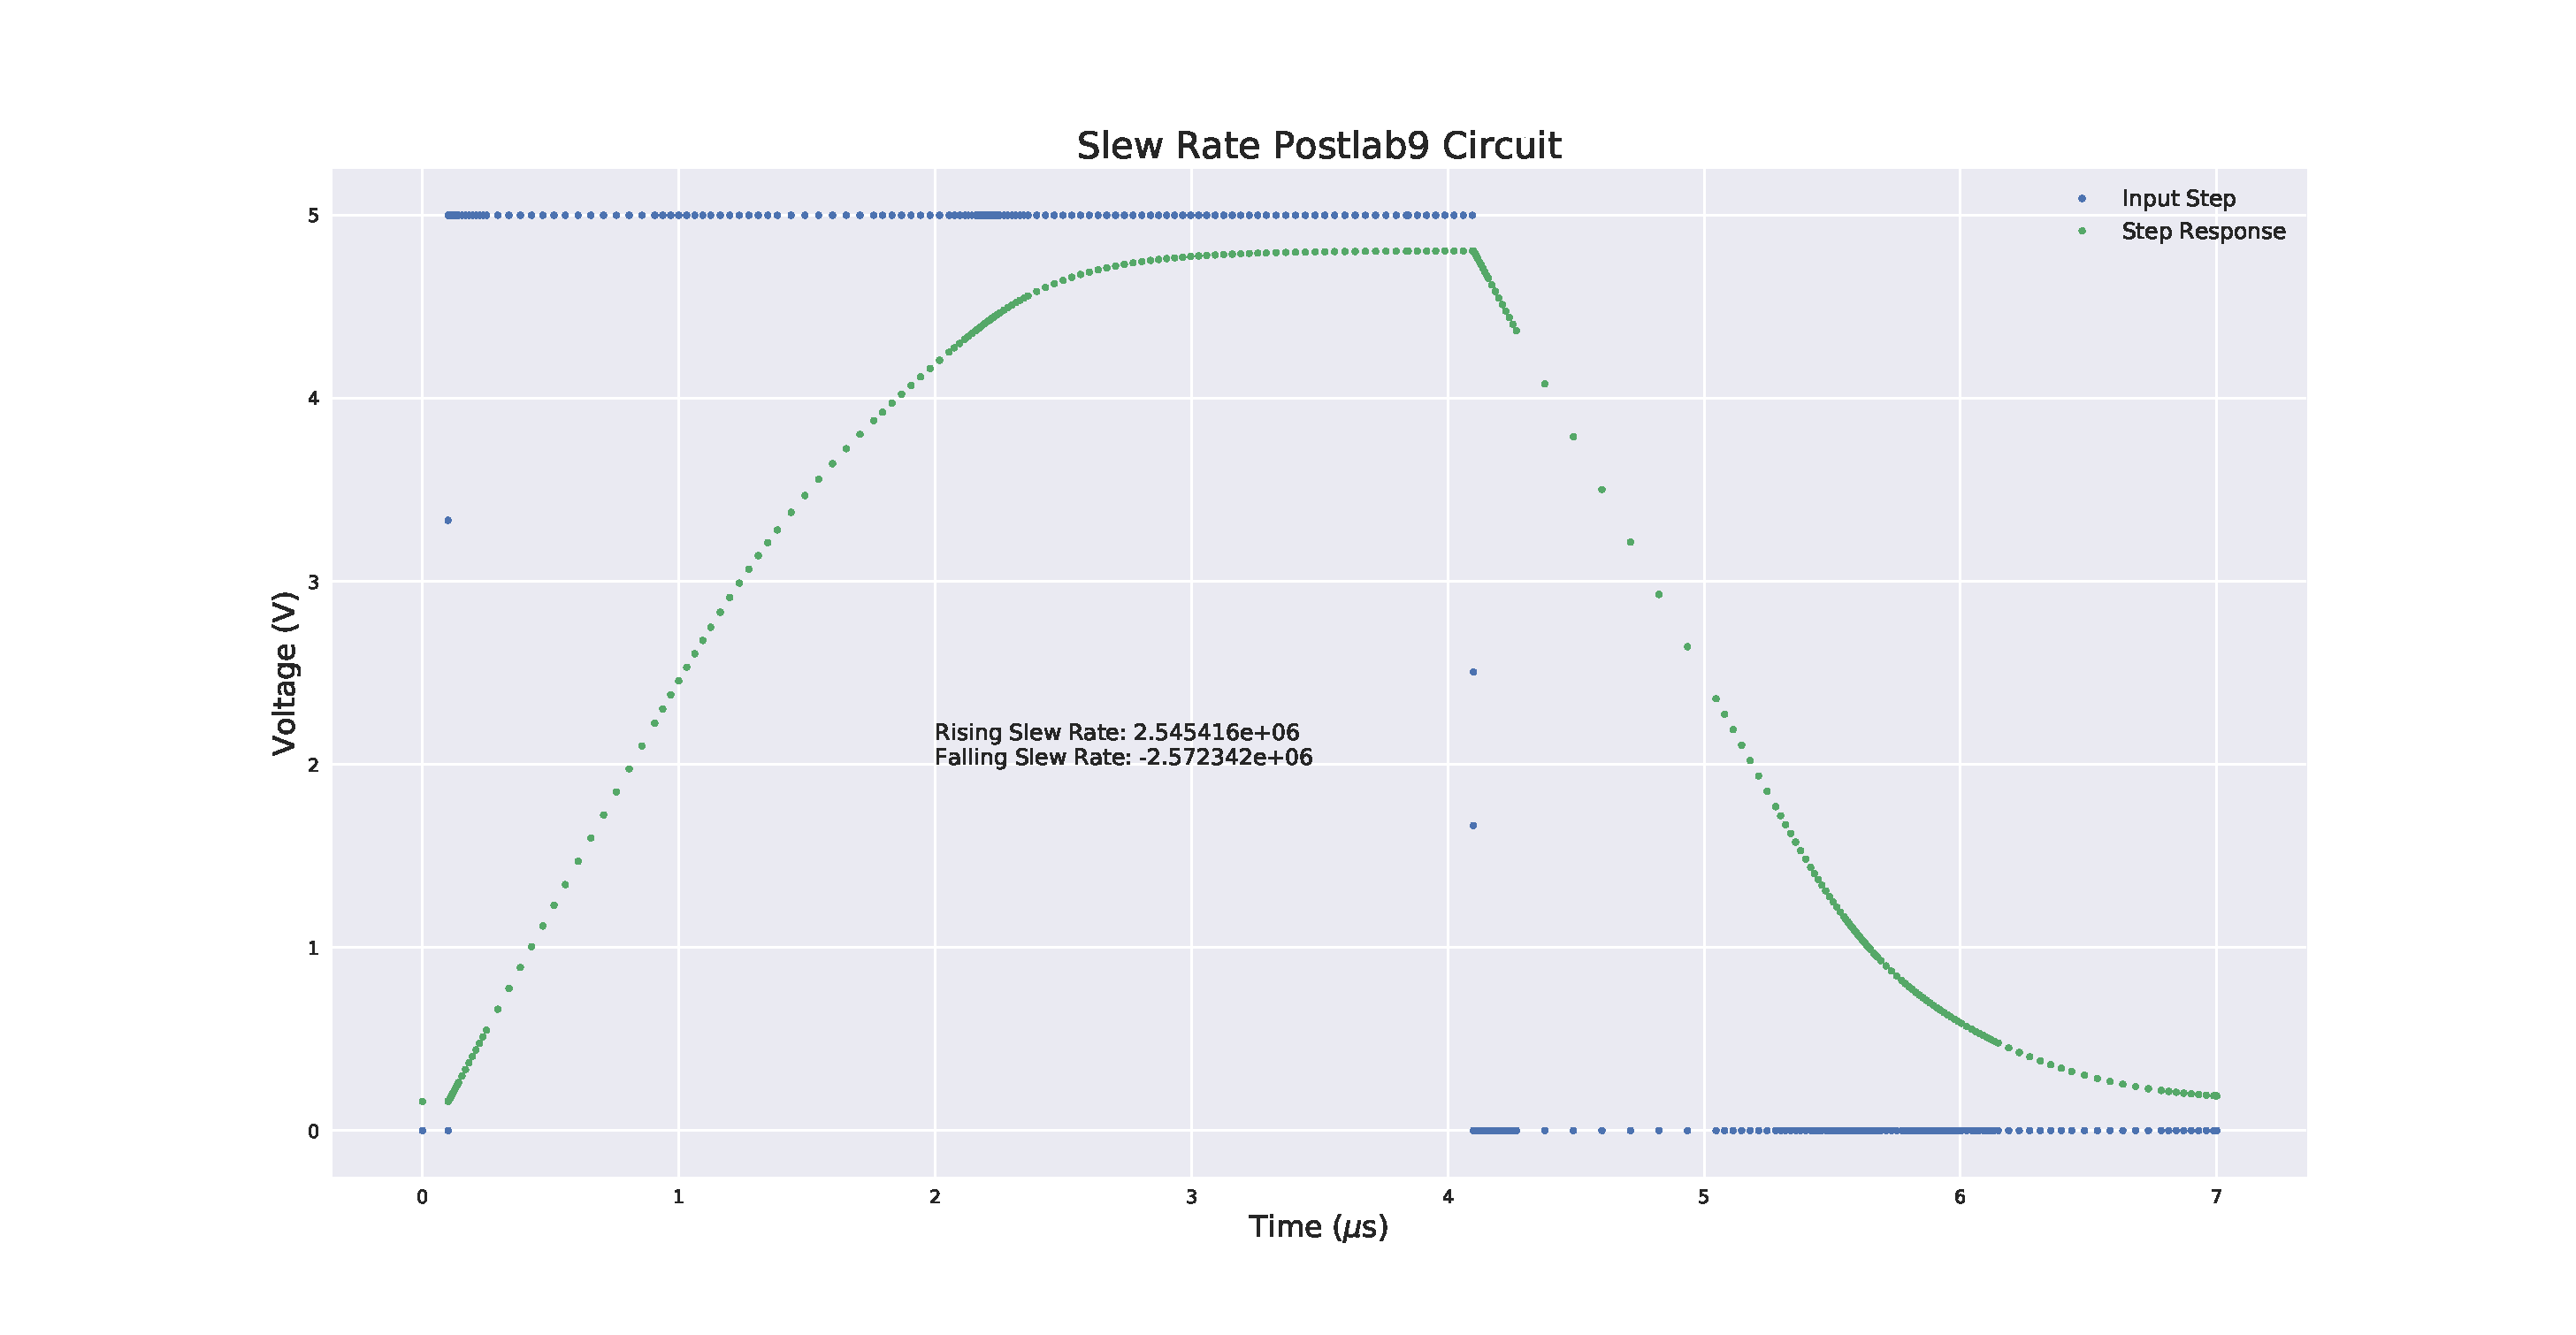
\includegraphics[width=\textwidth]{slew_rate_postlab9}
    \caption{Rising and Falling slew rate for Postlab9 Differential Amplifier Circuit.}
    \label{fig:postlab9}
\end{figure}

\section{Conclusion}

\end{document}
